\section{Terminology}
\frame{\tableofcontents[currentsection]}

\begin{frame}
  \frametitle{Terminology}
  \begin{itemize}
    \item Rightmost bit is called \emph{least significant bit} (MSB)
    \item Leftmost bit is called \emph{most significant bit} (LSB)
  \end{itemize}
  \begin{overprint}
    \onslide<1|handout:1>
    \structure{\texttt{uint8\_t}}
    \begin{center}
      \begin{tikzpicture}
        \draw (0,0) grid (8,1);
        \foreach[evaluate={\i-0.5} as \x] \i in {1,...,8} {
          \tikzmath{
            int \v;
            \v = random(0, 1);
          }
          \node at (\x, 0.5) {\v};
        }

        \node[anchor=north] (msb) at (0.5,-0.5) {most significant bit};
        \draw[-latex] (msb) -- (0.5,0);

        \node[anchor=north] (lsb) at (7.5,-0.5) {least significant bit};
        \draw[-latex] (lsb) -- (7.5,0);
      \end{tikzpicture}
    \end{center}

    \onslide<2|handout:0>
    \structure{\texttt{uint16\_t}}
    \begin{center}
      \begin{tikzpicture}
        \draw (0,0) grid[step=0.5cm] (8,0.5);
        \foreach[evaluate={\i/2-0.25} as \x] \i in {1,...,16} {
          \tikzmath{
            int \v;
            \v = random(0, 1);
          }
          \node[font=\tiny] at (\x, 0.25) {\v};
        }

        \node[anchor=north] (msb) at (0.25,-0.5) {most significant bit};
        \draw[-latex] (msb) -- (0.25,0);

        \node[anchor=north] (lsb) at (7.75,-0.5) {least significant bit};
        \draw[-latex] (lsb) -- (7.75,0);
      \end{tikzpicture}
    \end{center}

    \onslide<3|handout:0>
    \structure{\texttt{uint32\_t}}
    \begin{center}
      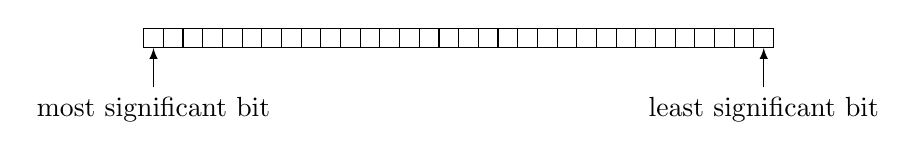
\begin{tikzpicture}
        \draw (0,0) grid[step=0.25cm] (8,0.25);
        \node[anchor=north] (msb) at (0.125,-0.5) {most significant bit};
        \draw[-latex] (msb) -- (0.125,0);

        \node[anchor=north] (lsb) at (7.875,-0.5) {least significant bit};
        \draw[-latex] (lsb) -- (7.875,0);
      \end{tikzpicture}
    \end{center}
  \end{overprint}
\end{frame}
